\chapter{Conditional Branching}
The branching we have done up until now has been unconditional branching: the branch instruction is always executed. This is highly limiting as the program can have only one flow. Conditional branching refers to the ability of the CPU to either take or ignore a branch instruction depending on some condition. This is very powerful as it allows the flow of the program to by variable depending on dynamic conditions. 

\section{Application Program Status Register}
The APSR is a special CPU register. It does not have a register number like the other registers and cannot be read or written by normal instructions. However this is a critically important register as it is the source of the conditions for the conditional branching. The APSR holds 4 flags:
\begin{description}
\item[Negative (N):] Set if the result of the last operations has was negative. In other words, the msb was a 1. This flag only has a meaning when treating data as signed numbers. 
\item[Zero (Z):] Set if all bits of the last operations were 0.
\item[Carry/Borrow (C):] Set if an \emph{unsigned} overflow occurred. Ie: the actual result of the computation exceeded the bounds of the 32-bit register when treated as an unsigned number.
\item[Two's Compliment Overflow (V):] Set if a \emph{signed} overflow occurred. Ie: the actual result of the computation exceeded the bounds of the 32-bit register when treated as a signed number. 
\end{description}

Together, these flags provide us with an abundance of information about the result of computations. We are able to ascertain basically any information about the relationship between arbitrary numbers by examining these flags. Not all instructions set the APSR flags. It is necessary to examine the details of the instruction in the Programming Manual in order to see whether the instruction sets the flags. Furthermore it may be necessary to examine the detailed workings of the instruction in the ARMv6-M Reference Manual in order to see which flags are set and how the settings of those flags is determined. However, in general instructions which set the flags have an \texttt{S} at the end of their name. Again (in general) arithmetic operations set/clear all APSR flags while logic operations set/clear only the \texttt{N} or \texttt{Z} flags. 

\section{Compare Instruction}
One of the key instructions used in the context of conditional branching is the compare (\texttt{CMP}) instruction. This instruction essentially subtracts two values from each other, disregards the result but updates the flags depending on the result. \texttt{CMP} takes either two registers or a register and an immediate value as operands. The CMP instruction is most often used to set the conditions which the conditional branch will depend on. This is due to the fact that a subtraction tells us a lot about the relationship between two numbers. For example, if the result of a subtraction sets the zero flag we know that the numbers being compared (subtracted) have the same value. Similarly, if the result of the subtraction of B from A clears the V flag it tell us that A is larger than B when viewed as signed numbers. 

The format of the \texttt{CMP} instruction is one of:
\begin{lstlisting}[fontadjust=true,frame=trBL]
CMP Rn, Rm
CMP Rn, #imm8
\end{lstlisting}
In the first case, the value of Rm is subtracted from Rn. In the seconds case, the 8-bit immediate number is subtracted from Rn.

\subsection{A note on the implementation of the subtract operation}
In order to minimize the hardware cost of the ALU circuitry, the subtract operations is implemented by adding the bitwise inverse of Rm to Rn, plus 1. You don't really have to worry about this other than to note that this implementation explains why the C or V flag is set when the numbers being compared are equal. For example, the subtraction of the number 42 from the number 42 corresponds to the addition of the numbers 42 and 4294967253 and 1. It should be apparent to you that this result is zero, but sets the carry flag. 


\section{Condition Code Suffixes} 
The branch (\texttt{B}) instruction is able to take optional condition code suffixes which specify whether or not the instruction will be executed depending on the state of the flags in the APRS. 
These suffixes are shown in \autoref{fig:cc_suff}. A suffix can be appended to the \texttt{B} instruction to turn it into a conditional branch. For example, \texttt{BEQ} will be taken if the result of the last computation produced a zero result. Similarly, \texttt{BNE} will be taken if the result was non-zero. 

The mnemonics for the suffixes are closely related to the compare operation. For example, the BGT (branch if greater than when treated as signed numbers) will be taken if the Rm operand of the CMP instruction is greater than the Rn operand when treated as signed numbers. This is why the CMP and B\{cc\}  instructions go so well together.

\begin{figure}
\centering
\includegraphics[page=40, clip=true, trim=110 130 60 434, width=\textwidth]{./stm32f0xx_programming_manual}
% left, bottom, right, top
\caption{Condition code suffixes and meanings. Source: Table 17, Programming Manual}
\label{fig:cc_suff}
\end{figure}

\section{Branching Based on Individual Bits}
Consider the case where we want to take a branch conditional on the case of a push button being pressed or not pressed. A push button is connected to a single pin which constitutes a single bit in the GPIO\_IDR. Hence, we need a way to make our branch conditional on a single bit being high or low. Put another way, we want to exclude all of the other bits in the IDR from influencing the branch. 

In order to achieve this we have to do two steps:
\begin{enumerate}
\item Mask out the bits which we are not interested in. Specifically, set them all to zero. This is done just as we saw earlier in \autoref{sec:set_clear_individual_bits}. We AND all of the bits with 0 except for the bit which we are interested in which we AND with 1.
\item Compare the result of the mask with 0. If the bit which we are interested in was 0 then the result of the AND will be 0. If the bit that we are interested in was 1 then the result of the AND will be non-zero. Note that this compare does not actually have to be done as the AND instruction sets or clears the zero flag.
\end{enumerate}
After those two steps (which can actually just be one step) we can take a conditional branch dependant on whether a single bit (a single push button) was set or cleared. 
